% !TEX program = xelatex
\documentclass[UTF8,12pt,a4paper]{ctexart}

\usepackage[a4paper,top=2.5cm,bottom=2.5cm,left=2.5cm,right=2.5cm]{geometry}
\usepackage{amsmath,amssymb,bm}
\usepackage{booktabs}
\usepackage{graphicx}
\usepackage{float}
\usepackage{caption}
\usepackage{subcaption}
\usepackage{hyperref}
\usepackage{listings}
\usepackage{xcolor}
%\usepackage{minted}
\usepackage{amsmath,amssymb} % 数学符号
\usepackage{fontspec}  % 自定义Consolas代码字体
% 代码环境宏包
\usepackage{pythonhighlight} % 或 mintex
\usepackage{ragged2e}
\pagestyle{plain}
\setCJKfamilyfont{zhsong}[AutoFakeBold=2.5]{SimSun}
\newcommand{\absbf}[1]{{\songti\bfseries #1}}

\hypersetup{colorlinks=true,linkcolor=black,citecolor=black,urlcolor=blue}
\linespread{1.35}
\setlength{\parindent}{2em}
\graphicspath{{../figures/}}
\ctexset{
  section = {format = {\songti\zihao{4}}},
  subsection = {format = {\songti\zihao{-4}}},
  subsubsection = {format = {\songti\zihao{-4}}}
}

\lstset{
  basicstyle=\ttfamily\small,
  breaklines=true,
  frame=single,
  backgroundcolor=\color{black!3},
  columns=fullflexible
}

\title{\songti 波浪能最大输出功率优化设计}
\author{}
\date{}

\begin{document}
\maketitle

\begin{abstract}
\songti
	振荡浮子式波能转换装置通过浮子与内部振子的相对运动提取波浪能，其输出功率受装置动力学响应和 PTO 阻尼参数共同影响。本文围绕垂荡与纵摇耦合条件下的运动响应计算和阻尼优化设计，建立分层动力学模型，并以稳态平均输出功率为统一评价指标给出参数选择方案。
	
	\absbf{针对问题一、二}，本文以浮子位移和振子位移为状态变量，建立二自由度耦合振动方程，分别讨论\absbf{线性阻尼}和\absbf{速度幂函数阻尼}两类 PTO 模式。线性阻尼情形下，利用\absbf{复振幅法}推导稳态解析解，并与 \absbf{Runge--Kutta 数值积分}结果进行对照，验证数值求解精度；非线性阻尼情形下，先在 $(\log c,\alpha)$ 平面上\absbf{粗扫描平均功率曲面}，确定高功率区域及单峰邻域，再以粗扫描最优点为初值采用 \absbf{Powell 下山法}局部精修，并对候选参数重新积分复算。计算结果表明，线性阻尼最优系数为 \absbf{$3.7421\times10^4\,\mathrm{N\cdot s/m}$}，有限窗口稳态平均功率为 \absbf{$226.60\,\mathrm{W}$}；非线性阻尼最优参数为 \absbf{$c=8.7065\times10^4,\alpha=0.3593$}，平均功率为 \absbf{$227.03\,\mathrm{W}$}，较线性最优结果略有提升。
	
	\absbf{针对问题三、四}，在进一步考虑浮子纵摇和振子相对纵摇后，本文保留浮子垂荡、振子沿中轴滑移、浮子纵摇和振子相对纵摇四个自由度，构建含三角函数投影、惯性耦合和重力矩耦合的\absbf{非线性几何模型}。针对给定阻尼参数，采用 \absbf{Radau 隐式积分法}求解系统响应；针对联合优化问题，先在 $(c_1,c_2)$ 参数平面作\absbf{二维粗扫描}，发现平均功率对垂荡阻尼更敏感且峰区呈带状分布，再以峰区内较优点启动\absbf{无导数局部优化}，并对最优候选解进行高精度稳态复算。最终得到最优垂荡阻尼系数 \absbf{$59846.67\,\mathrm{N\cdot s/m}$}、最优旋转阻尼系数 \absbf{$67472.34\,\mathrm{N\cdot m\cdot s}$}，对应稳态平均总功率 \absbf{$319.22\,\mathrm{W}$}。功率分解显示，在题给参数下\absbf{垂荡阻尼贡献占主导}，旋转阻尼功率占比较小，说明装置能量捕获能力主要由垂荡相对运动决定。
	
	本文还从稳态窗口选择、小角度适用性和几何有效范围等方面检验模型可靠性。结果说明，所建模型能够较好刻画振荡浮子式波能装置的主要动力学特征，所给阻尼参数优化策略具有较好的可复现性和工程解释性。
	

\songti 关键词：波浪能；耦合振动；非线性微分方程；平均功率；阻尼优化
\end{abstract}

\newpage

\section{问题重述与总体分析}

波浪能转换装置由浮子、振子、弹簧和阻尼器构成。波浪激励力使浮子产生垂荡或纵摇运动，浮子与内部振子之间的相对运动驱动 PTO 阻尼器做功，从而实现能量输出。题目要求在不同运动自由度和不同阻尼形式下，建立动力学模型并求解运动响应，进一步优化阻尼参数以最大化平均输出功率。

本文将四个子问题分为两类。问题一、二仅考虑垂荡运动，系统可抽象为浮子和振子的二自由度受迫耦合振动模型。问题一在给定阻尼参数下求运动响应；问题二在相同动力学框架下改变 PTO 阻尼参数，以稳态平均功率作为优化目标。问题三、四进一步考虑纵摇，系统自由度增至四个，几何关系导致方程中出现三角函数、变转动惯量和惯性耦合项，因此采用数值积分求解。问题四在问题三模型基础上同时优化垂荡线性阻尼和旋转阻尼。

本文采用的总体技术路线为：首先依据附件参数建立受力与力矩平衡方程；其次将高阶微分方程转化为一阶状态方程并用数值积分求解；最后通过稳态区间功率积分评价输出功率，并结合粗扫描与局部优化寻找最优阻尼参数。

\section{数据来源与参数处理}

结构参数来自附件4，包括浮子质量 $m_b=4866\,\mathrm{kg}$、振子质量 $m_z=2433\,\mathrm{kg}$、弹簧刚度 $k=80000\,\mathrm{N/m}$、海水密度 $\rho=1025\,\mathrm{kg/m^3}$、重力加速度 $g=9.8\,\mathrm{m/s^2}$ 等。水动力参数来自附件3，不同问题对应不同波浪圆频率、附加质量、兴波阻尼和激励力幅值。

浮子垂荡静水恢复力系数由水线面积给出：
\begin{equation}
  K_h=\rho g\pi r_b^2 .
  \label{eq:kh}
\end{equation}
在考虑纵摇时，静水恢复力矩系数取附件给定值 $K_\theta=8890.7\,\mathrm{N\cdot m}$。浮子纵摇转动惯量按照圆柱壳与圆锥壳表面积分配质量的近似公式计算；振子绕横向中心轴的转动惯量为
\begin{equation}
  I_z=\frac{1}{12}m_z(3r_z^2+h_z^2).
  \label{eq:iz}
\end{equation}

\section{模型假设与符号说明}

\subsection{模型假设}

为使模型在题给参数范围内可求解，作如下假设：

\begin{enumerate}
  \item 浮子只考虑题目指定方向的垂荡和纵摇运动，忽略横荡、横摇和艏摇等自由度。
  \item 海水密度恒定，浮子垂荡恢复力在小位移范围内可线性化为 $-K_h z_b$。
  \item PTO 阻尼器输出效率取为 1，即阻尼耗散功率等于可输出功率。
  \item 振子与浮子均视为刚体，弹簧和阻尼器只沿题设方向传递力或力矩。
  \item 问题三、四中纵摇角较小，并且浮子的顶端不会浸没，圆锥部分不会露出水面。
\end{enumerate}

\subsection{主要符号}

\begin{table}[H]
\centering
\caption{主要符号说明}
\begin{tabular}{lll}
\toprule
符号 & 含义 & 单位 \\
\midrule
$z_b,\dot z_b$ & 浮子垂荡位移与速度 & m, m/s \\
$z_z,\dot z_z$ & 振子沿中轴方向位移与速度 & m, m/s \\
$\theta_b,\dot\theta_b$ & 浮子纵摇角位移与角速度 & rad, rad/s \\
$\theta_z,\dot\theta_z$ & 振子相对纵摇角位移与角速度 & rad, rad/s \\
$m_b,m_z$ & 浮子质量、振子质量 & kg \\
$m_a,J_a$ & 垂荡附加质量、纵摇附加转动惯量 & kg, kg$\cdot$m$^2$ \\
$C_h,C_\theta$ & 垂荡、纵摇兴波阻尼系数 & N$\cdot$s/m, N$\cdot$m$\cdot$s \\
$k,k_\theta$ & 直线弹簧刚度、扭转弹簧刚度 & N/m, N$\cdot$m \\
$c_1,c_2$ & PTO 垂荡阻尼、旋转阻尼 & N$\cdot$s/m, N$\cdot$m$\cdot$s \\
$f,L$ & 波浪激励力、激励力矩幅值 & N, N$\cdot$m \\
$\omega$ & 入射波浪圆频率 & s$^{-1}$ \\
$P,\bar P$ & 瞬时输出功率、平均输出功率 & W \\
\bottomrule
\end{tabular}
\end{table}

\section{问题一：仅考虑垂荡运动的响应求解}

\subsection{二自由度垂荡模型}

\begin{figure}[H]
  \centering
  % 左图，占0.45行宽
  \begin{minipage}{0.45\textwidth}
    \centering
    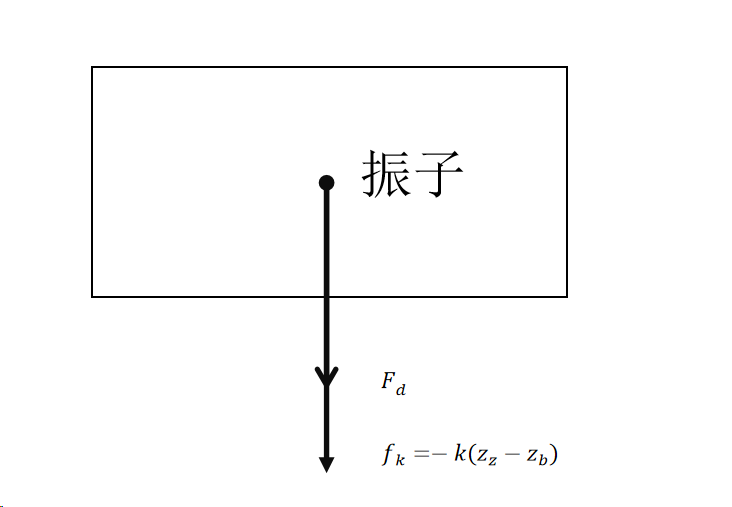
\includegraphics[width=\linewidth]{fig_problem1_model_1.png}
    \subcaption{振子}
  \end{minipage}
  % 两张图中间留间隙
  \hfill
  % 右图
  \begin{minipage}{0.45\textwidth}
    \centering
    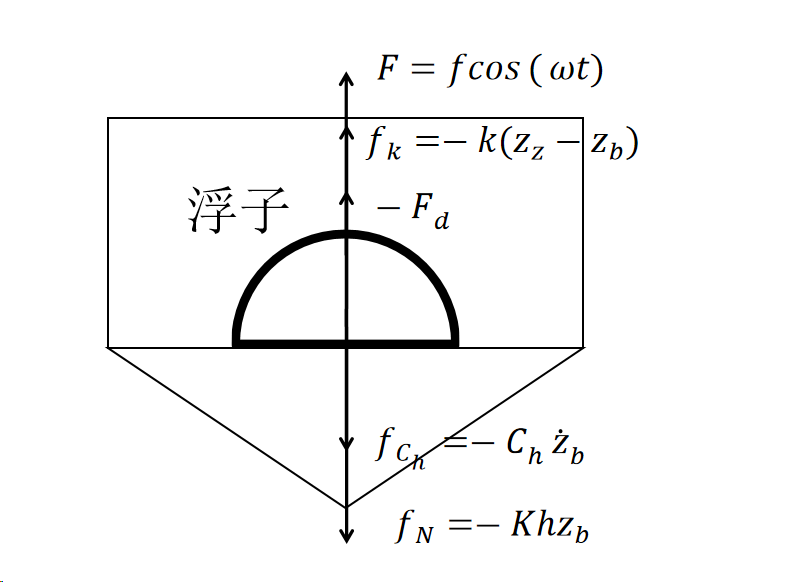
\includegraphics[width=\linewidth]{fig_problem1_model_2.png}
    \subcaption{浮子}
  \end{minipage}
  % 总图题
  \caption{系统受力分析}
  \label{fig:raw_resample}
\end{figure}

仅考虑垂荡时，取向下为正方向，浮子和振子的状态变量分别为 $z_b,z_z$。设相对位移为 $z_b-z_z$，相对速度为 $\dot z_b-\dot z_z$。线性阻尼情形下 PTO 阻尼力为
\begin{equation}
  F_d=c(\dot z_b-\dot z_z),
\end{equation}
非线性阻尼情形下阻尼系数随相对速度变化，本文采用题意对应形式
\begin{equation}
  F_d=c|\dot z_b-\dot z_z|^\alpha(\dot z_b-\dot z_z).
\end{equation}
弹簧的弹力为
\begin{equation}
  f_k=-k(z_z-z_b).
\end{equation}
令 $F_{\mathrm{PTO}}=f_k+F_d$，则浮子和振子垂荡方程为
\begin{align}
  (m_b+m_a)\ddot z_b
  &=f\cos\omega t-C_h\dot z_b-K_hz_b-F_{\mathrm{PTO}},\\
  m_z\ddot z_z&=F_{\mathrm{PTO}} .
\end{align}
初始时刻系统处于静水平衡状态，取 $z_b=z_z=\dot z_b=\dot z_z=0$。

\subsection{数值求解与结果}

将上述二阶方程化为一阶状态方程后，采用 Runge--Kutta 方法在 40 个波浪周期内积分，输出间隔为 $0.2\,\mathrm{s}$。图~\ref{fig:p1_response} 给出了线性阻尼和非线性阻尼下浮子、振子的垂荡响应。

\begin{figure}[H]
      \centering
      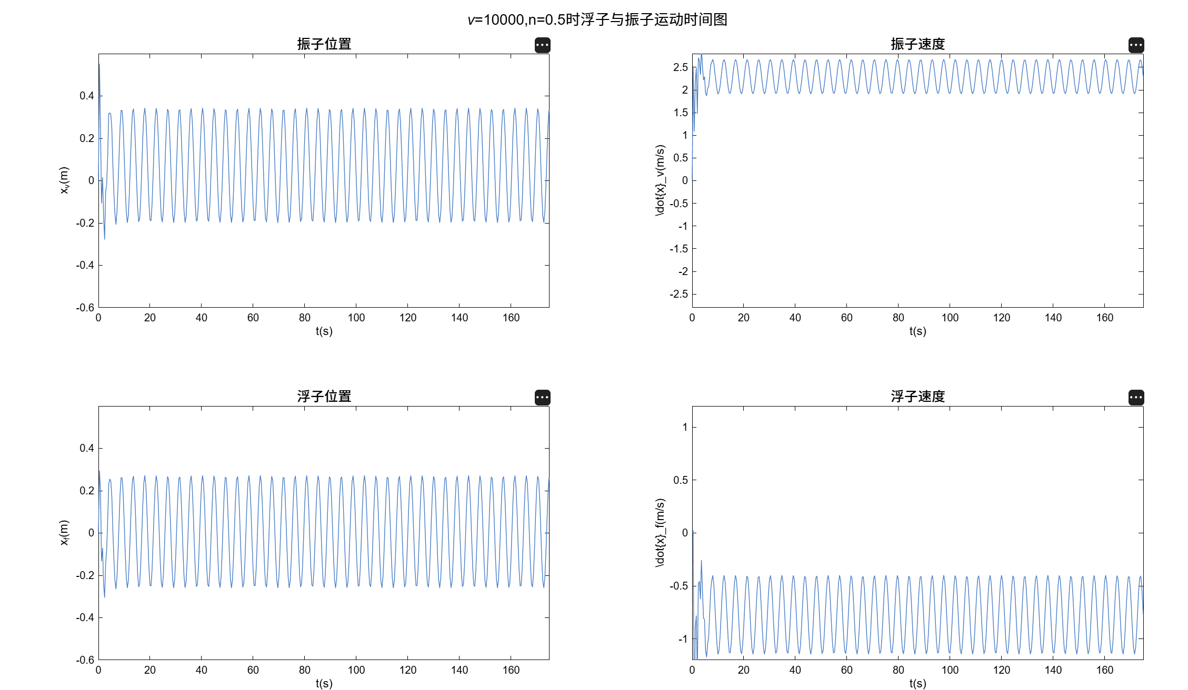
\includegraphics[width=0.75\linewidth]{fig+problem1_xiugai.png}
    \caption{问题一两种阻尼形式下的垂荡响应}
  \label{fig:p1_response}
\end{figure}

\begin{figure}[H]
    \centering
    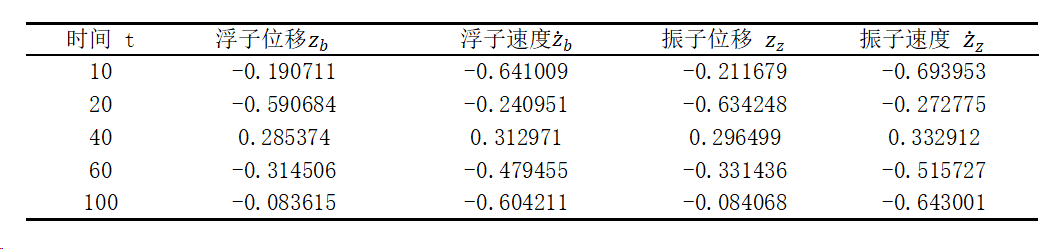
\includegraphics[width=0.75\linewidth]{fig_problem1_data.png}
    \caption{几个时间点的相关数据}
    \label{fig:placeholder3}
\end{figure}

由图可见，浮子在波浪激励下产生周期性垂荡，振子因惯性与 PTO 连接产生相位差，相对运动为阻尼器输出功率提供来源。非线性阻尼改变了相对速度较小时的阻尼强度，因此响应曲线与线性阻尼略有差异，但整体仍表现为受迫振动并逐渐进入稳定周期运动。

\section{问题二：垂荡阻尼参数优化}

\subsection{平均功率目标函数}

仅考虑垂荡时，PTO 输出功率来自阻尼器。线性阻尼的瞬时功率为
\begin{equation}
  P(t)=c(\dot z_b-\dot z_z)^2 .
\end{equation}
非线性阻尼下，阻尼力为 $c|v_r|^\alpha v_r$，其中 $v_r=\dot z_b-\dot z_z$，瞬时功率为
\begin{equation}
  P(t)=c|v_r|^{\alpha+2}.
\end{equation}
为避免初始过渡过程影响参数选择，本文对稳定区间内的功率作时间平均：
\begin{equation}
  \bar P(c,\alpha)=\frac{1}{T_2-T_1}\int_{T_1}^{T_2}P(t)\,dt .
  \label{eq:pavg}
\end{equation}

\subsection{优化方法}

对于线性阻尼，只有 $c$ 一个决策变量，先在 $[1,10^5]$ 上作对数网格粗搜索，再用黄金分割法精修。对于非线性阻尼，同时优化 $c$ 与 $\alpha$，先在 $(\log_{10}c,\alpha)$ 平面上粗扫描判断功率曲面，再采用 Powell 下山法和差分进化进行交叉验证。所有候选解均重新积分并计算稳态平均功率。

\subsection{优化结果}

由当前代码与结果表反推，线性阻尼最优系数为
\[
  c=37420.87\,\mathrm{N\cdot s/m},
\]
对应稳态平均功率约为 $226.60\,\mathrm{W}$。非线性阻尼最优参数为
\[
  c=87064.68,\qquad \alpha=0.3593,
\]
对应稳态平均功率约为 $227.03\,\mathrm{W}$。

\begin{figure}[H]
  \centering
  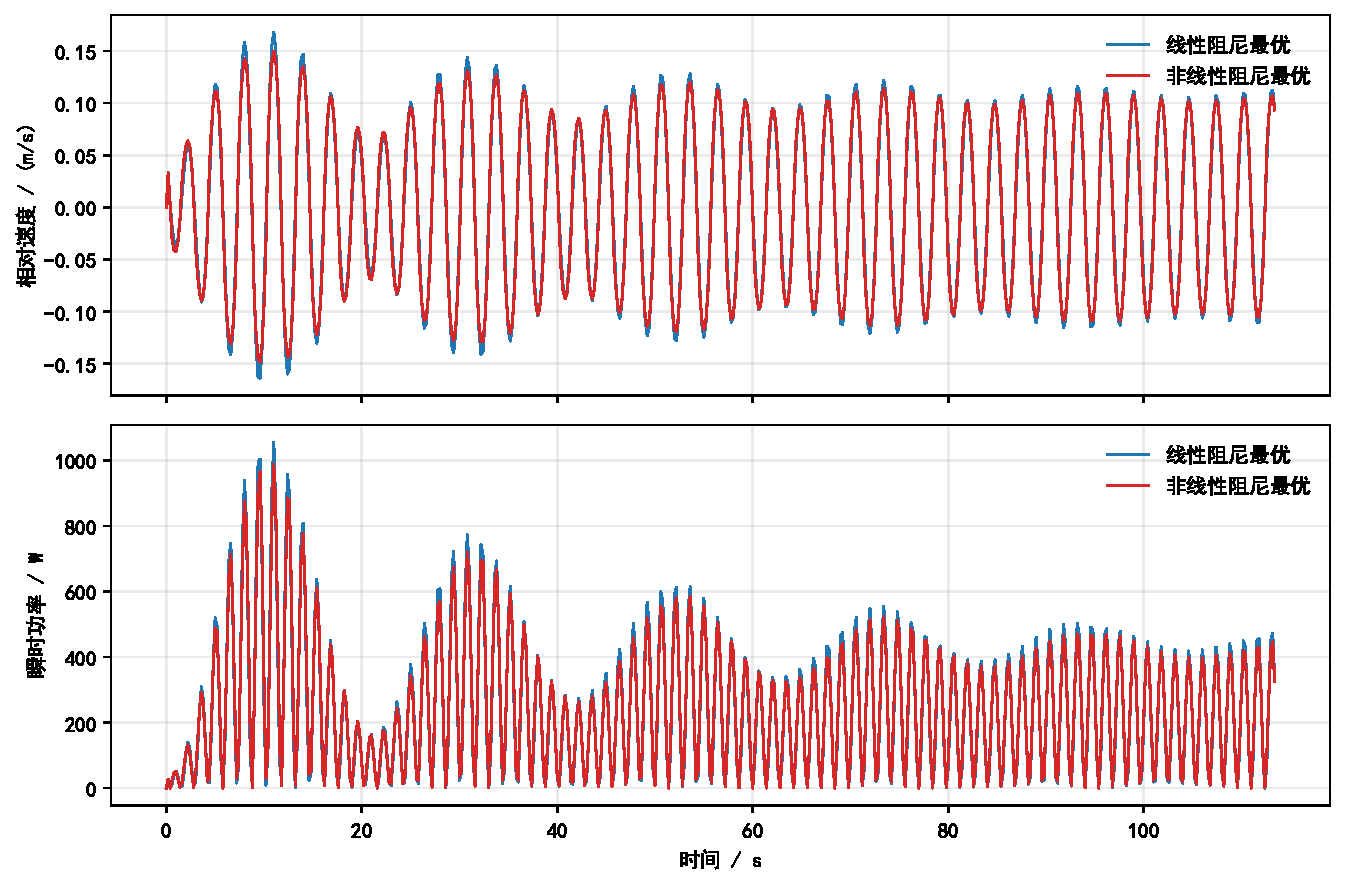
\includegraphics[width=0.90\textwidth]{fig_problem2_power.pdf}
  \caption{问题二最优阻尼参数下的相对速度与瞬时功率}
  \label{fig:p2_power}
\end{figure}

\begin{figure}[H]
  \centering
  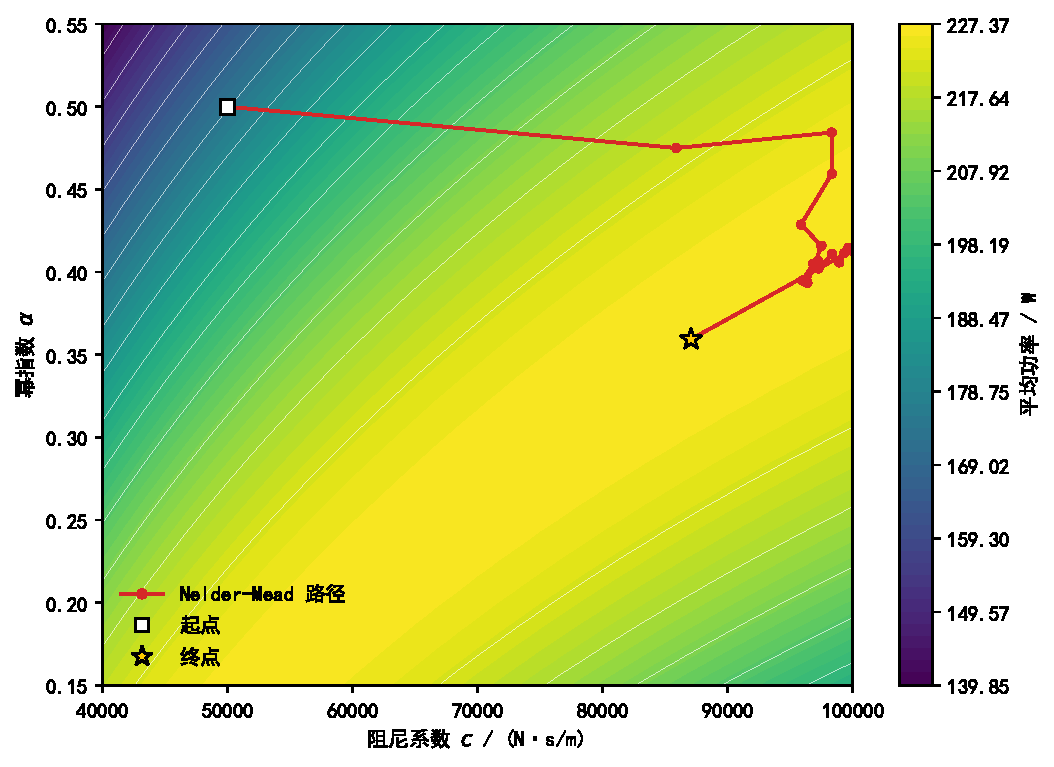
\includegraphics[width=0.58\textwidth]{fig_problem2_avg_power.pdf}
  \caption{问题二两种阻尼模式的稳态平均功率对比}
  \label{fig:p2_avg}
\end{figure}

从图~\ref{fig:p2_avg} 可以看出，非线性阻尼相对于线性阻尼的平均功率提升较小，但其通过幂指数调节不同相对速度区间的阻尼强度，使功率输出略有改善。

\section{问题三：垂荡--纵摇四自由度响应求解}

\subsection{非线性几何耦合模型}

\begin{figure}[H]
  \centering
  % 左图，占0.45行宽
  \begin{minipage}{0.45\textwidth}
    \centering
    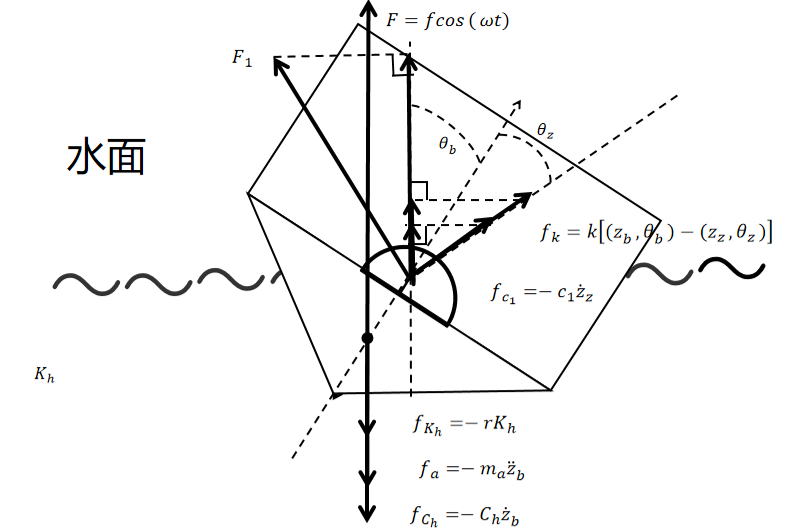
\includegraphics[width=\linewidth]{fig_problem3_xiugai.png}
    \subcaption{振子}
  \end{minipage}
  \hfill
  \begin{minipage}{0.45\textwidth}
    \centering
    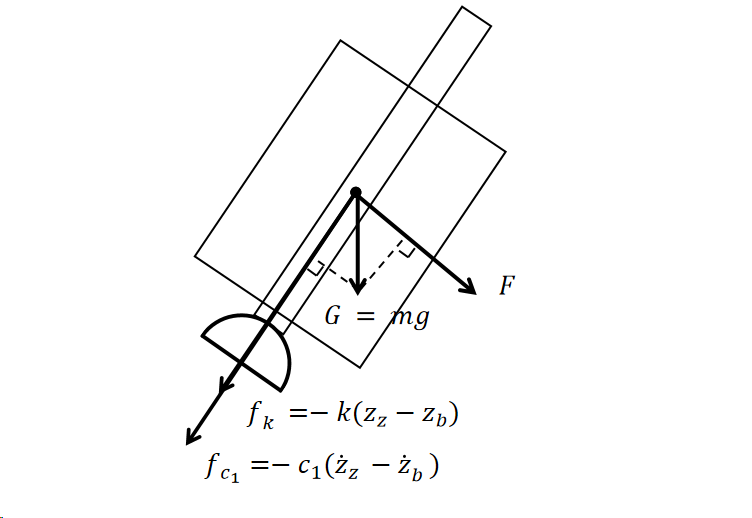
\includegraphics[width=\linewidth]{fig_problem3_model4.png}
    \subcaption{浮子}
  \end{minipage}
  % 总图题
  \caption{系统受力分析}
  \label{fig:raw_resample3}
\end{figure}

\begin{figure}
    \centering
    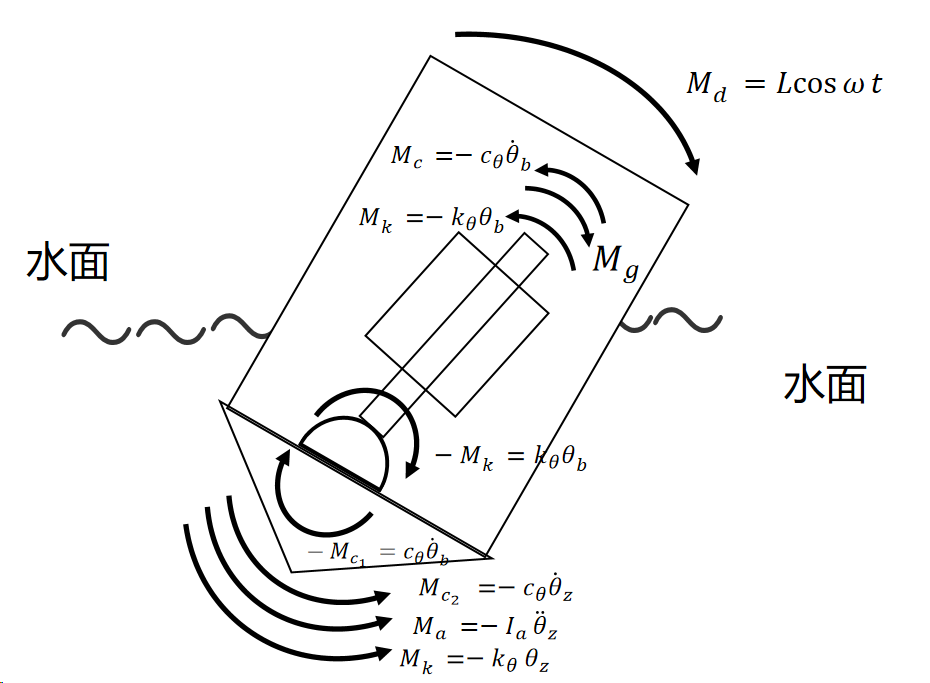
\includegraphics[width=0.75\linewidth]{fig_problem3_model5.png}
    \caption{力矩分析}
    \label{fig:placeholder6}
\end{figure}
问题三加入旋转阻尼器和扭转弹簧后，系统状态取为
\[
  \bm{x}=(z_z,z_b,\theta_z,\theta_b,\dot z_z,\dot z_b,\dot\theta_z,\dot\theta_b)^\mathsf{T}.
\]
其中 $z_z$ 表示振子沿浮子中轴方向的位置，$z_b$ 表示浮子垂荡位移，$\theta_z$ 表示振子相对浮子的纵摇角，$\theta_b$ 表示浮子纵摇角。振子中轴与竖直方向的夹角为
\[
  \phi=\theta_z+\theta_b .
\]

\iffalse
\begin{figure}[H]
  \centering
  % 左图，占0.45行宽
  \begin{minipage}{0.45\textwidth}
    \centering
    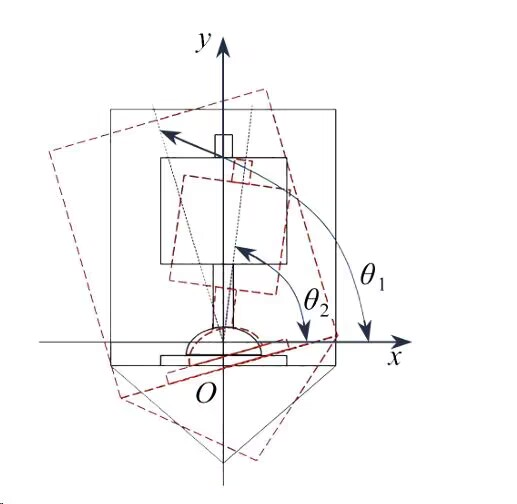
\includegraphics[width=\linewidth]{fig_problem3_model2.jpg}
    \subcaption{振子}
  \end{minipage}
  \hfill
  \begin{minipage}{0.45\textwidth}
    \centering
    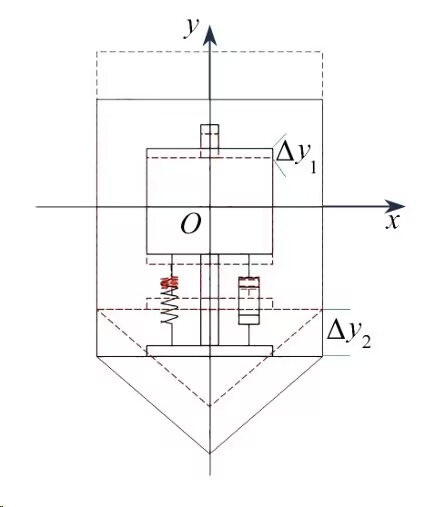
\includegraphics[width=\linewidth]{fig_problem3_model3.jpg}
    \subcaption{浮子}
  \end{minipage}
  % 总图题
  \caption{力矩分析}
  \label{fig:raw_resample2}
\end{figure}
\fi

浮子纵摇角加速度由力矩平衡给出：
\begin{equation}
  \ddot\theta_b=
  \frac{-K_\theta\theta_b-C_\theta\dot\theta_b+c_2\dot\theta_z
  +k_\theta\theta_z+L\cos\omega t}{I_b+J_a}.
  \label{eq:theta_b}
\end{equation}
振子相对纵摇的转动惯量随滑移位置变化：
\begin{equation}
  I_z^\ast=I_z+m_zz_z^2,
\end{equation}
对应角加速度为
\begin{equation}
  \ddot\theta_z=
  \frac{-c_2\dot\theta_z-k_\theta\theta_z+m_zgz_z\sin\phi}{I_z^\ast}
  -\ddot\theta_b .
  \label{eq:theta_z}
\end{equation}

垂荡方向上，浮子等效质量包含几何耦合项 $m_z\sin^2\phi$。在保留 AProblem 附录中惯性耦合项的形式下，可写为
\begin{equation}
  \ddot z_b=\frac{\mathcal{F}_b(z_z,z_b,\theta_z,\theta_b,\dot z_z,\dot z_b,\dot\theta_z,\dot\theta_b,t)}
  {m_b+m_a+m_z\sin^2\phi},
\end{equation}
其中 $\mathcal{F}_b$ 包含弹簧分力、阻尼分力、兴波阻尼、静水恢复力、波浪激励力以及振子垂直中轴方向惯性力。振子沿中轴方向加速度由
\begin{equation}
  \ddot z_z=\frac{-k(z_z-l_0)-c_1\dot z_z-m_zg\cos\phi
  -m_z\mathcal{A}_r}{m_z}
\end{equation}
给出，其中 $\mathcal{A}_r$ 为由浮子垂荡加速度和两角速度产生的径向惯性耦合项。

\subsection{求解设置与结果}

第三问中题给阻尼参数取 $c_1=10000\,\mathrm{N\cdot s/m}$、$c_2=1000\,\mathrm{N\cdot m\cdot s}$。由于方程含有较强非线性耦合并具有一定刚性，本文采用 Radau 隐式积分方法，误差控制为相对容差 $10^{-8}$、绝对容差 $10^{-10}$。初始条件取浮子处于静水平衡，振子沿中轴方向位于弹簧静平衡长度
\[
  z_z(0)=l_0-\frac{m_zg}{k}.
\]

\begin{figure}[H]
  \centering
  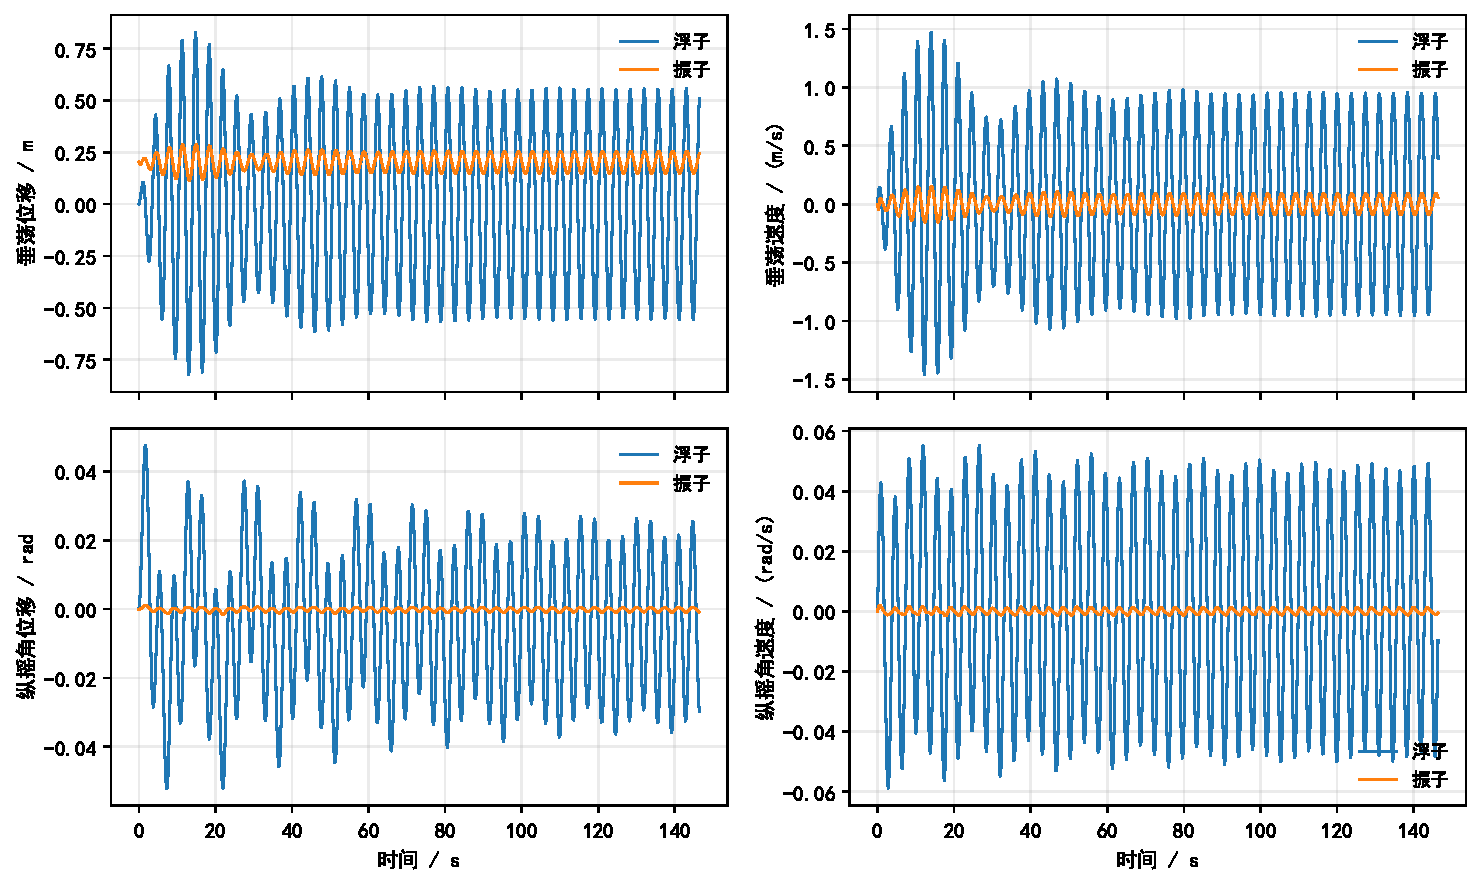
\includegraphics[width=0.95\textwidth]{fig_problem3_response.pdf}
  \caption{问题三给定阻尼参数下的四自由度响应}
  \label{fig:p3_response}
\end{figure}

\begin{figure}[H]
    \centering
    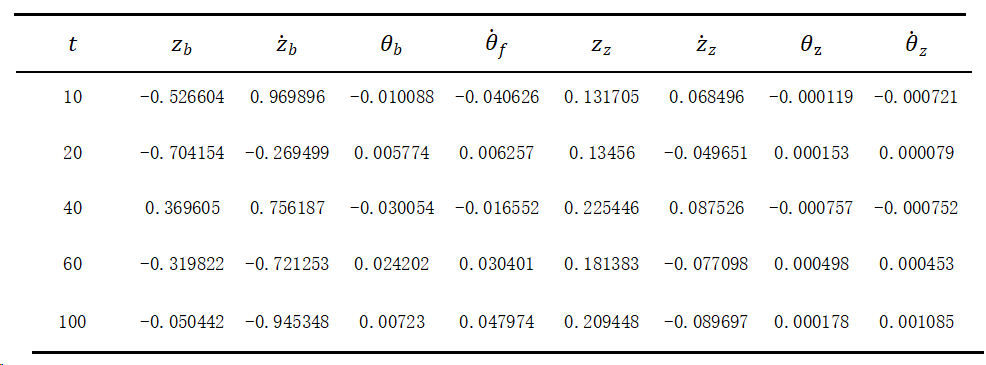
\includegraphics[width=0.9\linewidth]{fig_problem3_data.png}
    \caption{几个时间点的相关数据}
    \label{fig:placeholder4}
\end{figure}

由图~\ref{fig:p3_response} 可见，浮子垂荡响应幅值显著大于振子沿轴滑移幅值；纵摇响应中浮子角位移明显大于振子相对角位移。该结果说明在题给参数下，纵摇运动存在但幅值较小，后续功率优化中旋转阻尼功率可能不会成为总功率主导项。

\section{问题四：垂荡与旋转阻尼联合优化}

\subsection{优化目标}

问题四沿用问题三的四自由度非线性几何耦合模型，将垂荡阻尼 $c_1$ 与旋转阻尼 $c_2$ 同时作为决策变量。瞬时输出功率定义为
\begin{equation}
  P(t)=c_1\dot z_z^2+c_2\dot\theta_z^2,
  \label{eq:p4_inst}
\end{equation}
其中 $\dot z_z$ 为振子沿中轴方向相对滑移速度，$\dot\theta_z$ 为振子相对浮子的纵摇角速度。优化目标为稳定周期区间内的平均总功率：
\begin{equation}
  \max_{0\le c_1,c_2\le 10^5}
  \bar P(c_1,c_2)=
  \frac{1}{T_2-T_1}\int_{T_1}^{T_2}
  \left(c_1\dot z_z^2+c_2\dot\theta_z^2\right)\,dt .
  \label{eq:p4_obj}
\end{equation}

\subsection{粗扫描与局部优化}

本文先在 $[0,10^5]\times[0,10^5]$ 上进行二维粗扫描，得到功率峰值的大致区域；再以粗扫描最优点为初值，采用 Powell 无导数方法局部精修。优化阶段使用较低精度的数值积分以提高效率，最终候选参数再用高精度长时间积分复算。功率统计时丢弃初始过渡过程，仅使用稳定区间计算平均值。

\begin{figure}[H]
  \centering
  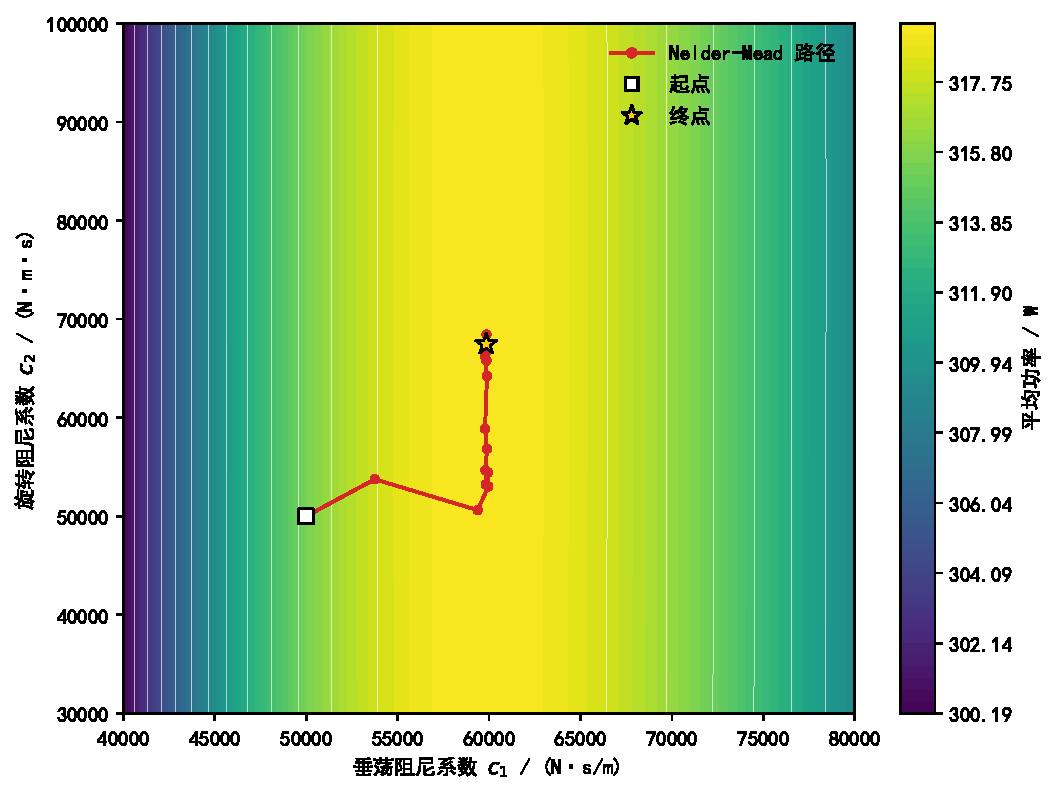
\includegraphics[width=0.78\textwidth]{fig_problem4_optimization_path_consistent.pdf}
  \caption{问题四垂荡阻尼与旋转阻尼的平均功率扫描结果}
  \label{fig:p4_surface}
\end{figure}

图~\ref{fig:p4_surface} 显示，功率对垂荡阻尼 $c_1$ 更敏感，而沿旋转阻尼 $c_2$ 方向变化较平缓。这与问题三中纵摇相对运动幅值较小的观察一致。

\subsection{最优结果与功率分解}

高精度复算得到
\begin{align*}
  c_1^\ast&=59846.67\,\mathrm{N\cdot s/m},\\
  c_2^\ast&=67472.34\,\mathrm{N\cdot m\cdot s},\\
  \bar P^\ast&=319.22345\,\mathrm{W}.
\end{align*}
其中垂荡平均功率为 $319.17646\,\mathrm{W}$，纵摇平均功率为 $0.04699\,\mathrm{W}$。因此本题参数下最优输出功率几乎全部由垂荡阻尼贡献。
\begin{figure}[H]
  \centering
  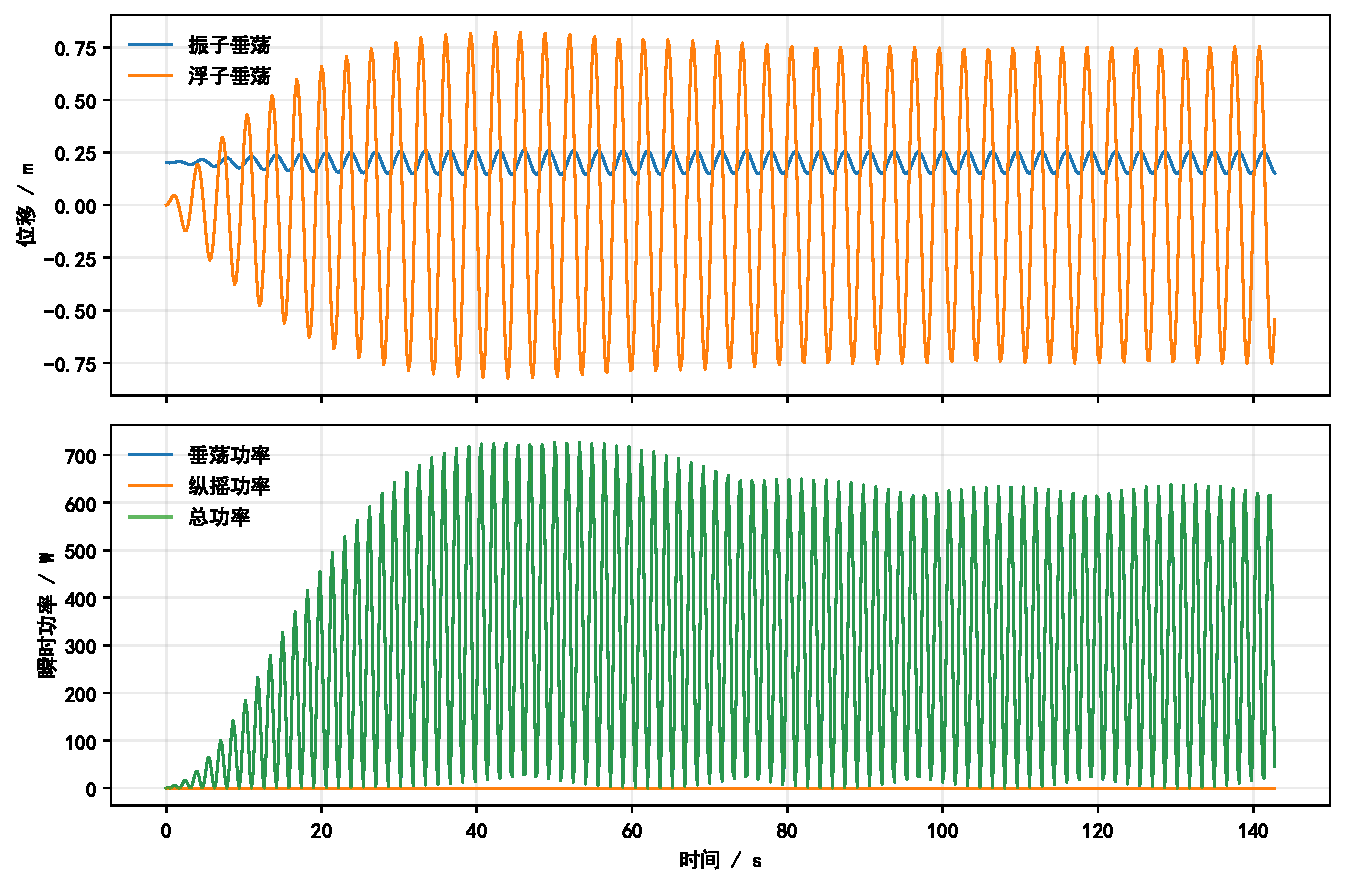
\includegraphics[width=0.90\textwidth]{fig_problem4_response_power.pdf}
  \caption{问题四最优阻尼参数下的响应与功率分解}
  \label{fig:p4_response}
\end{figure}

\section{模型检验、评价与改进}

\subsection{数值精度与解析解验证}

本文的计算过程主要包含三类近似：一是将二阶动力学方程转化为一阶状态方程后
进行数值积分，二是在稳态区间内对瞬时功率作时间平均，三是在阻尼参数空间内
进行最优值搜索。对于线性阻尼情形，方程具有线性常系数结构，可以利用解析解
对数值算法进行校验；对于非线性阻尼和垂荡--纵摇耦合情形，系统含速度幂函数、
三角函数和惯性耦合项，难以直接获得闭式解析解，因此需要依赖数值积分和优化。

本文采用如下精度口径：对运动响应，关注位移和速度时间序列的数值误差；对优化
结果，关注稳态平均功率和最优阻尼参数的稳定性。由于非线性模型难以给出严格的
全局解析误差上界，本文以线性可解析问题的逐时刻误差、线性功率解析值与数值值
的偏差，以及候选最优点复算结果共同确定数值精度。

以问题一的线性阻尼为例，令
\[
  \boldsymbol z=(z_b,z_z)^\mathsf{T},
\]
系统可写为
\begin{equation}
  M\ddot{\boldsymbol z}+C\dot{\boldsymbol z}+K\boldsymbol z
  =\boldsymbol f\cos\omega t .
  \label{eq:evaluation_linear_matrix}
\end{equation}
其稳态解可设为
\[
  \boldsymbol z_s(t)=
  \mathrm{Re}\left(\boldsymbol Z e^{i\omega t}\right),
\]
其中复振幅为
\begin{equation}
  \boldsymbol Z=
  \left(K-\omega^2M+i\omega C\right)^{-1}\boldsymbol f .
  \label{eq:evaluation_complex_amplitude}
\end{equation}
进一步将式~\eqref{eq:evaluation_linear_matrix} 化为一阶状态方程
\[
  \dot{\boldsymbol x}=A\boldsymbol x+\boldsymbol b\cos\omega t,
\]
可得到满足零初始条件的完整解析解
\begin{equation}
  \boldsymbol x(t)=
  \mathrm{Re}\left(\boldsymbol q e^{i\omega t}\right)
  +e^{At}\left[\boldsymbol x(0)-\mathrm{Re}(\boldsymbol q)\right],
  \quad
  \boldsymbol q=(i\omega I-A)^{-1}\boldsymbol b .
  \label{eq:evaluation_exact_state_solution}
\end{equation}
将式~\eqref{eq:evaluation_exact_state_solution} 与 Runge--Kutta 数值积分结果
逐时刻比较，在 $40$ 个波浪周期内，浮子位移最大绝对误差为
$1.07\times10^{-10}\,\mathrm{m}$，振子位移最大绝对误差为
$1.12\times10^{-10}\,\mathrm{m}$；在最后 $10$ 个周期内，两者最大绝对误差
分别降至 $1.68\times10^{-11}\,\mathrm{m}$ 和
$1.74\times10^{-11}\,\mathrm{m}$。相对于约 $0.4\,\mathrm{m}$ 的响应
幅值，最大相对误差约为 $10^{-10}$ 量级，说明数值积分误差远小于模型参数
和工程近似带来的误差。

对于问题二的线性阻尼优化，阻尼系数 $c$ 虽为决策变量，但每一个给定的
$c$ 仍对应一个线性受迫振动系统。因此可直接由复振幅得到稳态平均功率
\begin{equation}
  \bar P(c)=
  \frac{1}{2}c\omega^2|Z_b(c)-Z_z(c)|^2 .
  \label{eq:evaluation_linear_power}
\end{equation}
利用式~\eqref{eq:evaluation_linear_power} 作一维优化，得到
\[
  c^\ast=37193.81\,\mathrm{N\cdot s/m},
  \qquad
  \bar P_{\max}=229.33\,\mathrm{W}.
\]
数值积分优化得到的阻尼系数为
$c\approx37420.87\,\mathrm{N\cdot s/m}$，代入解析功率公式后得到
$\bar P=229.33\,\mathrm{W}$，与解析最优功率仅相差
$4.22\times10^{-3}\,\mathrm{W}$，相对差约为
$1.84\times10^{-5}$。因此，本文对位移响应保留到
$10^{-6}\,\mathrm{m}$、对平均功率保留到 $10^{-2}\,\mathrm{W}$ 是有
数值精度支撑的；阻尼系数则考虑到功率峰附近平台较平，报告到整数位或两位
小数均不会改变工程结论。

\subsection{模型适用范围检验}

模型评价不仅要关注数值解是否收敛，还要检验计算结果是否落在建模假设允许的
物理范围内。本文主要从稳态截取、浮子垂荡振幅和纵摇小角度三个方面进行检验。

首先，平均输出功率应在系统进入稳定受迫振动后计算。初始静止条件会引入暂态
响应，若将暂态区间纳入功率平均，容易使阻尼参数评价偏离长期运行状态。因此，
本文在优化和复算阶段均舍弃前期过渡过程，只对后段近周期响应计算平均功率。以
问题二线性阻尼情形为例，采用更长时间积分并取后段窗口平均时，平均功率收敛到
$229.33\,\mathrm{W}$，与复振幅解析稳态功率一致。这说明最终采用的功率评价
口径反映的是系统稳定受迫振动下的长期平均输出，而不是初始条件引起的暂态输出。

问题四中同样对稳态区间作了复核。该问题波浪周期为
\[
  T=3.17236\,\mathrm{s}.
\]
在最优阻尼参数下，计算时舍弃前 $25$ 个周期，即从 $79.31\,\mathrm{s}$ 后
开始统计稳态平均功率。比较 $25T$ 到 $35T$ 和 $35T$ 到 $45T$ 两个区间，
总平均功率分别为 $320.63\,\mathrm{W}$ 和 $319.61\,\mathrm{W}$，相对差约为
$0.32\%$。这表明在问题四的功率统计区间内，系统响应已基本进入稳定周期状态。
最终采用 $25T$ 到 $45T$ 的整体稳态区间计算，得到平均总功率
$319.22\,\mathrm{W}$。

其次，线性静水恢复力 $K_hz_b$ 隐含水线始终位于浮子圆柱段内，即水线面积
保持为 $\pi r_b^2$。由静水平衡可得浮子和振子的总排水体积为
\[
  V_0=\frac{m_b+m_z}{\rho}=7.12098\,\mathrm{m^3}.
\]
浮子下部圆锥体积为
\[
  V_{\mathrm{cone}}=\frac{1}{3}\pi r_b^2h_{\mathrm{cone}}
  =0.83776\,\mathrm{m^3}.
\]
因此平衡时圆柱段浸没高度为
\[
  h_0=\frac{V_0-V_{\mathrm{cone}}}{\pi r_b^2}
  =2.00001\,\mathrm{m}.
\]
题给圆柱高度为 $h_{\mathrm{cyl}}=3\,\mathrm{m}$，取 $z_b$ 向下为正，则
水线仍位于圆柱段内需要满足
\[
  -2.00001\le z_b\le 0.99999.
\]
若采用单一振幅阈值作保守检验，则
\[
  A_{\max}=0.99999\,\mathrm{m}.
\]
计算结果中，问题二浮子垂荡最大位移约为 $0.792\,\mathrm{m}$，问题三约为
$0.830\,\mathrm{m}$，问题四约为 $0.822\,\mathrm{m}$，均小于
$A_{\max}$。因此，题给参数和本文最优阻尼附近的响应没有使圆锥段露出水面，
也没有使水线进入圆柱顶部以上区域，线性静水恢复力的适用条件未被破坏。

最后，检验纵摇角是否属于小量。本文在第三、四问中使用了题给的线性纵摇附加
转动惯量、线性兴波阻尼矩和线性静水恢复力矩，其中浮子纵摇方程含有
$-K_\theta\theta_b-C_\theta\dot\theta_b$。这些水动力系数和恢复力矩均是在静平衡
姿态附近的小扰动意义下给出的，因此需要验证求得的纵摇响应没有进入大角度范围。
同时，本文在几何耦合项中仍保留 $\sin\phi$ 和 $\cos\phi$ 的非线性形式，并未
把三角函数整体替换为线性近似；小角度检验的作用，是说明线性纵摇水动力和恢复
力矩的使用是自洽的。

问题三中，整个计算区间内浮子和振子的最大纵摇角为
\[
  \theta_{\max}=0.05205\,\mathrm{rad}=2.98^\circ .
\]
若从后段稳态区间统计，最大纵摇角进一步降为
$0.04022\,\mathrm{rad}=2.30^\circ$。若在恢复力矩线性化或局部误差估计中采用
小角度近似，则由泰勒展开余项估计，
\[
  \frac{|\sin\theta-\theta|}{|\theta|}\lesssim\frac{\theta^2}{6},
  \qquad
  |1-\cos\theta|\lesssim\frac{\theta^2}{2}.
\]
取全区间最大角度 $\theta_{\max}=0.05205$，可得正弦近似相对误差不超过
$4.52\times10^{-4}$，余弦近似绝对误差不超过 $1.35\times10^{-3}$。
问题四的纵摇角更小，全区间最大纵摇角为
$0.04435\,\mathrm{rad}=2.54^\circ$；在 $25T$ 后的稳态统计区间内，最大
纵摇角为 $0.03160\,\mathrm{rad}=1.81^\circ$，此时正弦近似相对误差上界约为
$1.66\times10^{-4}$，余弦近似绝对误差上界约为 $4.99\times10^{-4}$。
因此，在题给激励和最优阻尼附近，纵摇响应始终保持小角度范围。

\subsection{优化结果稳定性分析}

阻尼参数优化的目标函数由受迫振动响应和功率积分共同决定。对于这类问题，最优
参数未必表现为尖锐的孤立点；若功率曲面在峰值附近较平，则一组参数都可能具有
近似相同的工程效果。因此，除了给出最优点，还需要分析最优结果的稳定性。

问题二线性阻尼情形可以由解析稳态功率函数直接判断最优区间。根据
式~\eqref{eq:evaluation_linear_power}，当
\[
  c\in[35561.29,38901.28]\,\mathrm{N\cdot s/m}
\]
时，稳态平均功率均不低于解析最优值的 $99.9\%$。这说明
$c=37193.81\,\mathrm{N\cdot s/m}$ 与数值优化得到的
$c=37420.87\,\mathrm{N\cdot s/m}$ 虽有差异，但对应平均功率几乎相同。
从工程角度看，线性阻尼参数可在上述区间内选择，而不必过度强调单点最优值。

问题二非线性阻尼优化得到
\[
  c=8.7065\times10^4,\qquad \alpha=0.3593,
\]
对应平均功率约为 $227.03\,\mathrm{W}$。与线性阻尼最优功率相比，非线性阻尼
在题给参数下带来的功率提升并不显著，说明该问题的主要优化空间仍来自阻尼强度
与系统固有响应之间的匹配，而非单纯依赖幂指数形式。由于非线性功率曲面存在
较平缓区域，幂指数和阻尼系数的数值不宜解释为绝对唯一的工程参数，而应理解为
在给定模型和频率下的一组有效匹配参数。

问题四中，最优阻尼参数为
\[
  c_1=59846.67\,\mathrm{N\cdot s/m},\qquad
  c_2=67472.34\,\mathrm{N\cdot m\cdot s}.
\]
稳态平均总功率为 $319.22\,\mathrm{W}$，其中垂荡阻尼贡献
$319.18\,\mathrm{W}$，旋转阻尼贡献仅 $0.047\,\mathrm{W}$。旋转阻尼功率
占总功率的比例约为
\[
  \frac{0.047}{319.22}=1.47\times10^{-4}.
\]
这与前述纵摇角较小的运动特征一致，也说明总功率主要由垂荡阻尼决定。因而在
问题四中，旋转阻尼最优值附近可能存在较大的等效选择空间；评价该结果时应更
重视总功率平台和垂荡阻尼匹配，而非将旋转阻尼的单点数值解释为唯一精确解。

\subsection{模型优点}

本文模型首先从受力和力矩平衡出发，变量定义和物理含义较为清晰。问题一、二
将系统抽象为浮子和振子的二自由度垂荡受迫振动模型，能够直接描述 PTO 弹簧和
阻尼器通过相对运动输出功率的机制；问题三、四进一步引入浮子纵摇、振子相对
转动以及振子沿浮子中轴滑移，使模型能够覆盖题目要求的主要运动自由度。

其次，本文没有完全依赖黑箱数值计算。在线性阻尼情形下，利用复振幅法和矩阵
指数形式给出解析解，并用解析结果对数值积分和线性功率优化进行验证；在非线性
阻尼和垂荡--纵摇耦合情形下，再采用数值积分方法求解。这样的处理既保留了线性
模型的精确性，又保证了后续复杂模型的可计算性。

再次，优化方法兼顾了全局搜索和局部精修。对阻尼参数先作粗扫描以观察功率曲面
形状和峰值区域，再用局部优化方法精修候选最优点，并通过高精度复算确认平均
功率。这种策略降低了局部优化对初值的依赖，也便于发现功率曲面较平坦时存在的
近似最优参数区间。

\subsection{模型局限与改进方向}

本文模型仍有若干局限。第一，模型采用固定静水面和线性静水恢复力，虽然前文已
验证本文计算结果没有超出水线位于圆柱段的适用范围，但当波浪激励进一步增大时，
水面相对浮子的位置和湿表面形状会发生明显变化，此时应引入瞬时水面高度和非线性
浮力模型。

第二，本文仅针对题给规则波和固定频率参数进行优化。实际海况往往由随机波谱或
多频波组成，最优阻尼可能随频率分布、波高和海况统计特征改变。后续可引入真实
波谱，对不同海况下的平均捕能效率进行评价，并寻找更具鲁棒性的阻尼参数。

第三，本文将 PTO 阻尼耗散功率等同于可输出功率，未考虑机械传动、电机转换、
控制策略和能量存储环节的损失。在工程应用中，应进一步建立 PTO 系统效率模型，
区分机械吸收功率和最终电功率。

第四，本文主要考虑平面内垂荡和纵摇运动，忽略横荡、横摇和艏摇等三维自由度。
对于实际海上装置，波浪入射方向和结构姿态可能导致更多自由度耦合。后续可将
本文的受力和力矩平衡框架推广到六自由度模型，以提高复杂海况下的适用性。


\newpage
\begin{thebibliography}{99}
\bibitem{landau}
朗道, 栗弗席兹. 力学[M]. 北京: 高等教育出版社, 2007.
\bibitem{simpson}
Weisstein E W. Simpson's Rule[EB/OL]. MathWorld--A Wolfram Web Resource.
\RaggedRight % 参考文献内柔和左对齐，自动断英文长词
\bibitem{rk}
Hairer E, Wanner G. Solving Ordinary Differential Equations  II: Stiff and Differential-Algebraic Problems[M]. Berlin: Springer, 1996.
\bibitem{wave}
Falnes J. Ocean Waves and Oscillating Systems[M]. Cambridge: Cambridge University Press, 2002.
\end{thebibliography}

\newpage
\appendix
\section{附录：文件列表与核心代码}

本文计算程序和结果表均存放于 \texttt{A题} 文件夹下。为便于复现，表~\ref{tab:appendix_files}
列出本文提交和复核所需的主要文件。其中 \texttt{problem1.py} 至 \texttt{problem4.py}
对应四个子问题的主程序，两个 analytic 文件用于线性情形的解析解校验和功率复核。

\begin{table}[H]
  \centering
  \caption{主要程序文件和结果文件}
  \label{tab:appendix_files}
  \small
  \begin{tabular}{p{0.34\textwidth}p{0.56\textwidth}}
    \toprule
    文件名 & 作用说明 \\
    \midrule
    \texttt{problem1.py} & 求解问题一中线性阻尼和非线性阻尼下的二自由度垂荡响应。\\
    \texttt{problem2.py} & 对问题二的线性阻尼系数及非线性阻尼参数进行功率优化。\\
    \texttt{problem3.py} & 求解问题三中垂荡--纵摇四自由度非线性几何耦合模型。\\
    \texttt{problem4.py} & 对问题四的垂荡阻尼和旋转阻尼进行联合优化。\\
    \texttt{problem1\_analytic\_check.py} & 构造问题一线性阻尼情形的时域解析解，并与数值解比较。\\
    \texttt{problem2\_linear\_analytic.py} & 利用复振幅法计算问题二线性阻尼的稳态平均功率和最优阻尼。\\
    \texttt{result1-1.xlsx} & 问题一线性阻尼情形的计算结果表。\\
    \texttt{result1-2.xlsx} & 问题一非线性阻尼情形的计算结果表。\\
    \texttt{result3.xlsx} & 问题三给定阻尼参数下的四自由度响应结果表。\\
    \bottomrule
  \end{tabular}
\end{table}

以下仅给出各程序中与建模和优化直接相关的核心代码片段。为控制附录篇幅，参数定义、文件读写、
绘图语句和重复性辅助代码均已省略。

\subsection{问题一：二自由度垂荡响应}

\begin{lstlisting}[language=Python,caption={问题一垂荡运动方程与数值积分核心片段}]
def ode_system(t, x, c_damp, nonlinear=False, alpha=0.5):
    z_b, zb_dot, z_z, zz_dot = x
    rel_disp = z_b - z_z
    rel_vel = zb_dot - zz_dot
    if nonlinear:
        f_damp = c_damp * abs(rel_vel) ** alpha * rel_vel
    else:
        f_damp = c_damp * rel_vel
    f_pto = k_spring * rel_disp + f_damp
    zb_ddot = (f_amp*np.cos(omega*t) - C_wave*zb_dot
               - K_hydro*z_b - f_pto) / (m_b + m_add)
    zz_ddot = f_pto / m_z
    return [zb_dot, zb_ddot, zz_dot, zz_ddot]
\end{lstlisting}

\subsection{问题二：阻尼参数优化}

\begin{lstlisting}[language=Python,caption={问题二平均功率与非线性阻尼优化核心片段}]
def damping_power(c, alpha, rv):
    return c * np.abs(rv) ** (alpha + 2)

def search_nonlinear_surface(c_range=(1e-2, 100000), alpha_range=(0.0, 1.0),
                             n_c=36, n_alpha=31):
    log_bounds = (np.log10(c_range[0]), np.log10(c_range[1]))
    log_grid = np.linspace(log_bounds[0], log_bounds[1], n_c)
    alpha_grid = np.linspace(alpha_range[0], alpha_range[1], n_alpha)
    records, best = [], (-np.inf, None, None)
    for a in alpha_grid:
        for log_c in log_grid:
            c = 10 ** log_c
            p_val = rk4_power(c, a, n_total=32, n_drop=16)
            records.append((c, a, p_val))
            if p_val > best[0]:
                best = (p_val, c, a)

    def objective(x):
        log_c, alpha = x
        c = 10 ** log_c
        return -rk4_power(c, alpha, n_total=36, n_drop=18)

    x0 = np.array([np.log10(best[1]), best[2]])
    powell = minimize(objective, x0, method="Powell",
                      bounds=[log_bounds, alpha_range])
    de = differential_evolution(objective, bounds=[log_bounds, alpha_range])
    # 对粗扫、Powell 和差分进化的候选点统一长时间复算。
\end{lstlisting}

\subsection{问题三：四自由度非线性耦合模型}

\begin{lstlisting}[language=Python,caption={问题三非线性几何耦合方程与 Radau 积分核心片段}]
def ode_system(t, x):
    z_z, z_b, th_z, th_b, zz_dot, zb_dot, thz_dot, thb_dot = x
    angle = th_z + th_b
    sin_a = np.sin(angle)
    cos_a = np.cos(angle)
    thb_ddot = (-K_pitch*th_b - C_pitch*thb_dot
                + c_rotary*thz_dot + k_torsion*th_z
                + L_amp*np.cos(omega*t)) / (I_b + J_add)
    Iz_eff = I_z + m_z * z_z**2
    thz_ddot = (-c_rotary*thz_dot - k_torsion*th_z
                + m_z*g*z_z*sin_a) / Iz_eff - thb_ddot
    m_eff = m_b + m_add + m_z * sin_a**2
    zb_ddot = (
        k_linear*(z_z-l0+m_z*g/k_linear)*cos_a + c_linear*zz_dot*cos_a
        - C_heave*zb_dot + f_amp*np.cos(omega*t) - K_heave*z_b
        + sin_a*(m_z*(z_z*thz_ddot + 2*zz_dot*thz_dot
        + z_z*thb_ddot + 2*zz_dot*thb_dot) - m_z*g*sin_a)
    ) / m_eff
    zz_ddot = (
        -k_linear*(z_z-l0) - c_linear*zz_dot - m_z*g*cos_a
        - m_z*(-z_z*thz_dot**2 + zb_ddot*cos_a
        - z_z*thb_dot**2 - 2*z_z*thb_dot*thz_dot)
    ) / m_z
    return [zz_dot, zb_dot, thz_dot, thb_dot,
            zz_ddot, zb_ddot, thz_ddot, thb_ddot]

sol = solve_ivp(ode_system, (0, 40*T_period), x0, t_eval=t_eval,
                method="Radau", rtol=1e-8, atol=1e-10)
\end{lstlisting}

\subsection{问题四：垂荡与旋转阻尼联合优化}

\begin{lstlisting}[language=Python,caption={问题四平均功率计算和局部优化核心片段}]
def average_power(c_linear, c_rotary, n_periods=45, drop_periods=25):
    sol = solve_response(c_linear, c_rotary, n_periods=n_periods)
    t = sol.t
    mask = t >= drop_periods * T_period
    zz_dot = sol.y[4, mask]
    thz_dot = sol.y[6, mask]
    t = t[mask]
    p_heave = c_linear * zz_dot ** 2
    p_pitch = c_rotary * thz_dot ** 2
    p_linear = np.trapezoid(p_heave, t) / (t[-1] - t[0])
    p_rotary = np.trapezoid(p_pitch, t) / (t[-1] - t[0])
    return PowerResult(c_linear, c_rotary, p_linear+p_rotary,
                       p_linear, p_rotary)

def coarse_scan():
    values = np.linspace(0.0, 100000.0, 11)
    rows = []
    for c1 in values:
        for c2 in values:
            rows.append(average_power(c1, c2).__dict__)
    return pd.DataFrame(rows).sort_values("p_total", ascending=False)

def refine_from(best):
    cache = {}
    def objective(v):
        c1, c2 = v
        key = (round(c1), round(c2))
        if key not in cache:
            cache[key] = average_power(c1, c2)
        return -cache[key].p_total
    opt = minimize(objective, [best.c_linear, best.c_rotary],
                   method="Powell", bounds=[(0, 1e5), (0, 1e5)])
    return average_power(opt.x[0], opt.x[1])
\end{lstlisting}

\subsection{线性问题的解析校验}

\begin{lstlisting}[language=Python,caption={问题一线性阻尼时域解析解核心片段}]
def analytic_solution(times):
    A, b = state_matrices()
    q = np.linalg.solve(1j*omega*np.eye(4) - A, b)
    x0 = np.zeros(4)
    x_ss_0 = np.real(q)
    exact = []
    for t in times:
        x_steady = np.real(q * np.exp(1j*omega*t))
        x_exact = x_steady + expm(A*t).dot(x0 - x_ss_0)
        exact.append(x_exact)
    return np.asarray(exact), q
\end{lstlisting}

\begin{lstlisting}[language=Python,caption={问题二线性阻尼稳态功率解析优化核心片段}]
def complex_amplitude(c):
    M = np.array([[m_b + m_add, 0], [0, m_z]], dtype=complex)
    C = np.array([[C_w + c, -c], [-c, c]], dtype=complex)
    K = np.array([[K_h + k_s, -k_s], [-k_s, k_s]], dtype=complex)
    F = np.array([f_amp, 0], dtype=complex)
    return np.linalg.solve(K - omega**2*M + 1j*omega*C, F)

def analytic_power(c):
    z = complex_amplitude(c)
    return 0.5 * c * omega**2 * abs(z[0] - z[1]) ** 2
\end{lstlisting}


\end{document}
